% IEEE conference paper. Compile in Overleaf or TeX Live (IEEEtran ships with both).
% Build: pdflatex main -> bibtex main -> pdflatex main -> pdflatex main
\documentclass[conference]{IEEEtran}

%
% --- common packages (IEEEtran loads very few by default) ---
%
\usepackage{graphicx}
\usepackage{amsmath,amssymb}
\usepackage{booktabs}
\usepackage{array}
\usepackage{url}
\usepackage{xcolor}


\usepackage[colorlinks,allcolors=blue]{hyperref}
\usepackage[capitalize]{cleveref}

\title{Generalizable Wearable Stress Detection from\\ Heart-Rate Variability: A Subject-Independent Study}

\author{\IEEEauthorblockN{Aravind Marri}
\IEEEauthorblockA{\textit{Independent Researcher}\\
contact@aravindmarri.com}}

\begin{document}
\maketitle

\begin{abstract}
Wearable devices increasingly promise to detect psychological stress from
physiological signals, yet reported accuracies are often inflated by
subject-dependent evaluation that lets the same person appear in both training
and test sets. We study how well a stress detector built on heart-rate
variability (HRV) alone, a signal available on consumer wrist wearables,
generalizes to \emph{unseen} people. Using the public WESAD dataset, we extract
seven standard time- and frequency-domain HRV features from 60-second windows of
wrist photoplethysmography (PPG) and evaluate four classifiers under strict
Leave-One-Subject-Out (LOSO) cross-validation on a binary baseline-versus-stress
task. HRV features achieve a macro-F1 of 0.87 and AUROC of 0.95 (logistic
regression), far above a heart-rate-only baseline (macro-F1 0.54), and the best
model is also the most stable across subjects. Ablations show that variability
features carry stress information beyond heart rate alone, that rate and time-domain
variability together are strongest, and that longer windows help. A specificity check
shows the detector separates stress from amusement, a different high-arousal state
(macro-F1 0.84), rather than tracking arousal alone, and we report per-subject bootstrap
confidence intervals. Critically, a
validity check against WESAD's synchronized ECG shows the wrist sensor recovers heart
rate but \emph{not} beat-to-beat HRV (near-zero RMSSD/SDNN agreement), so these
features are better described as pulse-rate variability than as validated HRV. We
release a reproducible pipeline (pinned tooling, a per-window manifest, and
per-subject predictions). Our results give a realistic, subject-independent reference
point, and a cautionary note on what wrist sensing can and cannot measure.
\end{abstract}

\begin{IEEEkeywords}
heart-rate variability, stress detection, wearable sensing, photoplethysmography,
affective computing, subject-independent evaluation
\end{IEEEkeywords}

\section{Introduction}
\label{sec:intro}
Chronic and acute psychological stress are strongly linked to cardiovascular,
metabolic, and mental-health outcomes, and continuous, unobtrusive stress
monitoring is one of the most requested features of consumer wearables. Among the
signals these devices can capture, heart-rate variability (HRV), the variation in
time between consecutive heartbeats, has a well-established physiological link to
autonomic nervous system activity and stress~\cite{taskforce1996hrv,shaffer2017hrv,kim2018hrv}.
Crucially, HRV can be derived from the photoplethysmography (PPG) sensor already
present in virtually every wrist wearable, making it an attractive, low-cost basis
for on-device stress detection.

A large body of work reports high accuracy for wearable stress detection. However,
many studies evaluate with record- or window-level cross-validation that places
windows from the \emph{same} subject in both training and test folds. Because
physiology is highly person-specific, such protocols measure how well a model
memorizes an individual rather than how well it generalizes to a new user, the
setting that actually matters when a model ships to millions of devices. The gap
between subject-dependent and subject-independent performance is frequently large,
yet the former is still widely reported.

In this paper we ask a deliberately conservative question: \emph{using only HRV,
how well can a stress detector trained on a labeled population generalize to an
unseen person?} We study this on the public WESAD dataset~\cite{schmidt2018wesad}
using strict Leave-One-Subject-Out (LOSO) cross-validation. Our contributions are:
\begin{itemize}
  \item A subject-independent benchmark of HRV-based stress detection on wrist PPG,
        compared against explicit majority-class and heart-rate-only baselines and
        reported with per-subject variability (\cref{sec:main}).
  \item A feature ablation isolating mean heart rate, time-, and frequency-domain
        variability (including a variability-only model), reported with stress recall
        and specificity, plus an analysis-window sweep (\cref{sec:ablations}).
  \item A stress-specificity analysis (a three-class baseline/stress/amusement task and a
        direct stress-versus-amusement task) showing the detector captures stress rather
        than generic arousal, reported with per-subject bootstrap confidence intervals
        (\cref{sec:specificity}).
  \item A signal-validity analysis comparing PPG-derived HRV against WESAD's
        synchronized ECG, with a motion split, showing the wrist sensor captures rate
        but not beat-to-beat HRV (\cref{sec:validity}).
  \item A reproducible, open pipeline (pinned tooling, a per-window manifest, and
        per-subject predictions) and a protocol for consumer-device validation
        (\cref{sec:conclusion}).
\end{itemize}

\section{Related Work}
\label{sec:related_work}
\textbf{HRV and stress.} The autonomic correlates of HRV are well documented: the
measurement standards of~\cite{taskforce1996hrv} and the metric overview
of~\cite{shaffer2017hrv} define the time- and frequency-domain indices used
throughout this work, and a meta-analysis~\cite{kim2018hrv} confirms that acute
stress systematically reduces several HRV indices. These findings motivate HRV as
a physiologically grounded feature set rather than an opaque signal.

\textbf{Wearable stress detection.} WESAD~\cite{schmidt2018wesad} introduced a
multimodal benchmark combining chest and wrist sensors and has become a standard
testbed. Wrist-only approaches such as~\cite{gjoreski2017stress} and the broad
survey of~\cite{can2019stress} report strong results across devices and signals.
Our work is complementary and deliberately narrow: we isolate the HRV channel
available on commodity wrist devices and measure it under a strict
subject-independent protocol, providing a realistic reference point rather than a
best-case multimodal number.

\cref{tab:related} situates our setup against representative WESAD-based results.
Reported accuracies approaching $0.9$ typically rely on multimodal fusion (notably
electrodermal activity) and often on the chest device; by isolating the wrist HRV
channel under strict LOSO we obtain a comparable binary accuracy from a single,
commodity-available signal, forgoing the headroom that richer modalities provide.
The figures are not directly comparable, as the studies differ in sensors, class
definitions, and reported metric; the table is included only to locate our operating
point within the literature.

\begin{table}[t]
  \centering
  \caption{Representative WESAD-based stress detection under subject-independent
  (LOSO) evaluation. Accuracies are as reported by each source and are \emph{not}
  directly comparable (differing sensors, classes, and metrics). EDA: electrodermal
  activity; ACC: accelerometer.}
  \label{tab:related}
  \begin{tabular}{@{}p{2.3cm}p{2.2cm}p{1.4cm}c@{}}
    \toprule
    Study & Device / signals & Features & Bin.\ acc. \\
    \midrule
    Schmidt et al.~\cite{schmidt2018wesad} & chest+wrist, multimodal (ECG, EDA, EMG, resp., temp., ACC, BVP) & many & up to 0.93 \\
    Gjoreski et al.~\cite{gjoreski2017stress} & wrist, multimodal (BVP, EDA, temp., ACC) & many & $\approx$0.85 \\
    \textbf{This work} & wrist PPG only & 7 HRV & 0.885 \\
    \bottomrule
  \end{tabular}
\end{table}

\section{Methodology}
\label{sec:method}
\subsection{Dataset}
We use WESAD~\cite{schmidt2018wesad}, which contains synchronized physiological
recordings from 15 subjects (identifiers S2--S11 and S13--S17). We use the wrist
device's PPG/blood-volume-pulse (BVP) channel, sampled at 64~Hz, together with the
protocol labels. We frame the task as binary classification of \emph{baseline}
versus \emph{stress} conditions, excluding transient and other states.

\subsection{Feature Extraction}
Each recording is divided into 60-second windows with a 30-second stride. A window
is retained only if at least 90\% of its samples share a single label, which is
then used as the window label. For each window, the PPG signal is cleaned and
systolic peaks are detected with NeuroKit2~\cite{makowski2021neurokit}; inter-beat
intervals (IBIs) outside the physiologically plausible range of 300--2000~ms are
discarded, and windows with fewer than twelve beats are dropped. From the IBI
series we compute seven standard HRV features: four time-domain
(mean heart rate, SDNN, RMSSD, pNN50) and three frequency-domain (LF and HF band
power and the LF/HF ratio). Frequency-domain features are obtained by cubic
interpolation of the tachogram to 4~Hz followed by a Welch power spectral density
estimate, integrated over the LF (0.04--0.15~Hz) and HF (0.15--0.40~Hz) bands.
This procedure yields 869 labeled windows (562 non-stress, 307 stress), 55--61 per
subject.

\subsection{Models and Evaluation}
We compare four classifiers: a mean-heart-rate-only baseline (logistic regression
on a single feature), logistic regression, a random forest (300 trees), and a
small multilayer perceptron (hidden layers 32--16), all on standardized features.
Standardization statistics are fit on the training split only.

We evaluate with Leave-One-Subject-Out (LOSO) cross-validation: in each of the 15
folds, one subject is held out for testing and the remaining fourteen are used for
training, so no window from the test subject is ever seen during training. We
report mean accuracy, macro-F1, and AUROC across folds, as well as the standard
deviation of per-subject macro-F1 as a measure of how consistently a model
generalizes across individuals.

\section{Experiments}
\label{sec:experiments}

\subsection{Main Results}
\label{sec:main}
\cref{tab:main} reports LOSO performance. The heart-rate-only baseline performs
poorly (macro-F1 0.54, AUROC 0.67), confirming that mean heart rate alone is a
weak stress indicator across subjects. Adding the full HRV feature set yields a
large improvement: logistic regression reaches macro-F1 0.87 and AUROC 0.95, with
the small MLP essentially tied. Beyond mean performance, logistic regression also
has the lowest per-subject F1 standard deviation (0.094), indicating that it
generalizes most consistently to unseen individuals, a desirable property for a
model intended to ship to a diverse user base. \cref{fig:models} summarizes the
comparison.

To quantify uncertainty across individuals, we bootstrap the per-subject macro-F1
(random forest, 5000 resamples over the 15 subjects): the mean is 0.82 with a 95\%
confidence interval of $[0.74, 0.90]$, and per-subject values range from 0.41 for the
hardest subject to 0.98 for the easiest (median 0.86). The interval sits well above
chance, but the spread confirms that a few individuals remain substantially harder than
the rest.

\begin{table}[t]
  \centering
  \caption{LOSO results on WESAD (baseline vs.\ stress). Best per column in bold.}
  \label{tab:main}
  \begin{tabular}{@{}lcccc@{}}
    \toprule
    Model & Acc. & Macro-F1 & AUROC & F1 std.\ \\
    \midrule
    mean-HR only (baseline) & 0.689 & 0.541 & 0.668 & 0.191 \\
    Logistic Regression     & \textbf{0.885} & \textbf{0.873} & \textbf{0.952} & \textbf{0.094} \\
    Random Forest           & 0.838 & 0.823 & 0.905 & 0.159 \\
    Small MLP               & 0.882 & 0.870 & 0.948 & 0.116 \\
    \bottomrule
  \end{tabular}
\end{table}

\begin{figure}[t]
  \centering
  \IfFileExists{figures/fig_models.png}
    {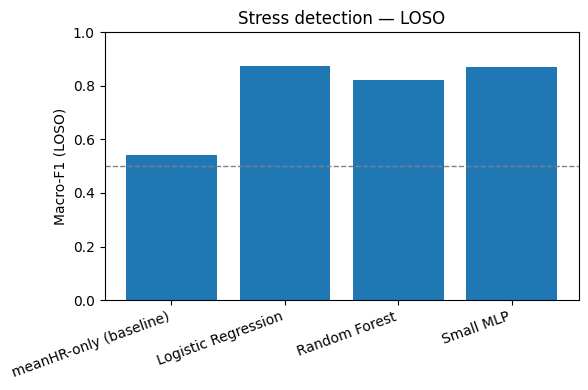
\includegraphics[width=\linewidth]{figures/fig_models.png}}
    {\fbox{\parbox{0.9\linewidth}{\centering\vspace{1.5em} Place \texttt{figures/fig\_models.png} here\\ (downloaded from the Colab run).\vspace{1.5em}}}}
  \caption{Macro-F1 by model under LOSO cross-validation. The dashed line marks
  chance-level macro-F1.}
  \label{fig:models}
\end{figure}

\begin{figure}[t]
  \centering
  \IfFileExists{figures/fig_per_subject.png}
    {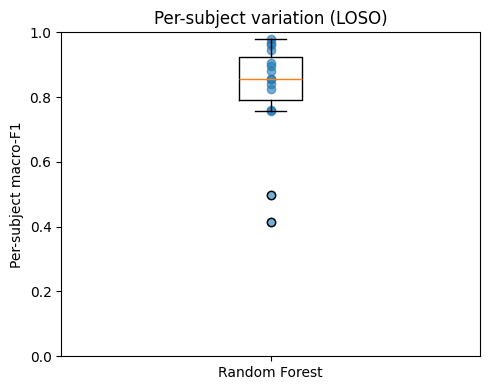
\includegraphics[width=0.85\linewidth]{figures/fig_per_subject.png}}
    {\fbox{\parbox{0.9\linewidth}{\centering\vspace{1.5em} Place \texttt{figures/fig\_per\_subject.png} here.\vspace{1.5em}}}}
  \caption{Per-subject macro-F1 for the random forest under LOSO, showing the spread
  across the 15 held-out subjects.}
  \label{fig:per_subject}
\end{figure}

\subsection{Ablations}
\label{sec:ablations}
\textbf{What carries the signal?} \cref{tab:abl} isolates each feature group under
LOSO (logistic regression, our headline model) against a majority-class baseline.
Every HRV-based model beats the trivial 0.39 macro-F1 baseline. A mean-HR-only model
is weak (macro-F1 0.54) and rarely flags stress (stress recall 0.27). Variability
features \emph{without} mean HR are substantially better (macro-F1 0.71), confirming
that beat-to-beat variability carries stress information beyond rate. The strongest
models, however, combine rate with time-domain variability (macro-F1 0.87);
frequency-domain features alone are weak (macro-F1 0.64), consistent with poor
low-frequency resolution at a 60-second window. \cref{fig:importance} shows mean heart
rate and the time-domain indices dominate feature importance.

\begin{table}[t]
  \centering
  \caption{Feature ablation under LOSO (logistic regression, baseline vs.\ stress),
  with a majority-class baseline. Str.\ rec.: stress recall; Non-str.\ spec.:
  non-stress specificity. Best per column in bold.}
  \label{tab:abl}
  \begin{tabular}{@{}lccccc@{}}
    \toprule
    Feature set & Acc. & F1 & AUROC & Str.\ rec. & Non-str.\ spec. \\
    \midrule
    Majority baseline        & 0.647 & 0.393 & --    & 0.000 & \textbf{1.000} \\
    Mean-HR only             & 0.689 & 0.541 & 0.668 & 0.270 & 0.914 \\
    Variability only (no HR) & 0.756 & 0.714 & 0.762 & 0.578 & 0.854 \\
    Frequency-domain only    & 0.716 & 0.644 & 0.766 & 0.412 & 0.882 \\
    Time-domain (incl.\ HR)  & 0.885 & 0.872 & 0.952 & 0.828 & 0.915 \\
    All features             & \textbf{0.885} & \textbf{0.873} & \textbf{0.952} & \textbf{0.835} & 0.912 \\
    \bottomrule
  \end{tabular}
\end{table}

\begin{figure}[t]
  \centering
  \IfFileExists{figures/fig_importance.png}
    {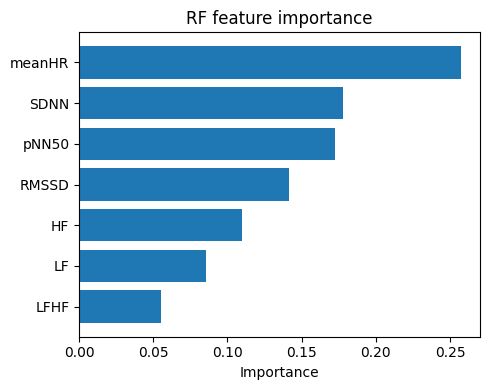
\includegraphics[width=0.85\linewidth]{figures/fig_importance.png}}
    {\fbox{\parbox{0.9\linewidth}{\centering\vspace{1.5em} Place \texttt{figures/fig\_importance.png} here.\vspace{1.5em}}}}
  \caption{Random forest feature importances. Mean heart rate and the time-domain HRV
  indices dominate.}
  \label{fig:importance}
\end{figure}

\textbf{Window length.} \cref{tab:ablwin} varies the analysis window. Accuracy and
macro-F1 increase across the tested window lengths, from 30~s (macro-F1 0.79) to
120~s (macro-F1 0.86), as longer windows contain more beats and yield more stable
HRV estimates. This
exposes a latency--accuracy trade-off for real-time use: shorter windows respond
faster but are noisier.

\begin{table}[t]
  \centering
  \caption{Window-length ablation (Random Forest, LOSO).}
  \label{tab:ablwin}
  \begin{tabular}{@{}cccc@{}}
    \toprule
    Window (s) & Acc. & Macro-F1 & AUROC \\
    \midrule
    30  & 0.808 & 0.787 & 0.883 \\
    60  & 0.838 & 0.823 & 0.905 \\
    120 & 0.869 & 0.855 & 0.918 \\
    \bottomrule
  \end{tabular}
\end{table}

\subsection{Stress specificity: three classes and stress vs.\ amusement}
\label{sec:specificity}
A detector that merely responds to physiological \emph{arousal} would confuse stress
with other high-arousal states. We probe specificity in two ways. First, we extend the
task to three classes (baseline, stress, amusement) under LOSO with the random forest.
Macro-F1 is 0.52 (accuracy 0.69), well above the 0.24 majority-class baseline.
\cref{tab:conf3} shows \emph{where} errors fall. Stress is recovered well (recall 0.83)
and is almost never mistaken for amusement (only 1.3\% of stress windows), while amusement
is largely absorbed into baseline (recall 0.03). The model therefore does not treat stress
as generic arousal; instead, amusement's wrist signature sits close to baseline and is the
hard class, consistent with amusement being a milder affective manipulation than the
stress protocol.

\begin{table}[t]
  \centering
  \caption{Three-class LOSO confusion (random forest), row-normalised so the diagonal is
  per-class recall. Stress is well separated and rarely confused with amusement; amusement
  collapses into baseline.}
  \label{tab:conf3}
  \begin{tabular}{@{}lccc@{}}
    \toprule
    True $\downarrow$ / Pred.\ $\rightarrow$ & baseline & stress & amusement \\
    \midrule
    baseline  & \textbf{0.80} & 0.15 & 0.05 \\
    stress    & 0.15 & \textbf{0.83} & 0.01 \\
    amusement & 0.89 & 0.08 & \textbf{0.03} \\
    \bottomrule
  \end{tabular}
\end{table}

Second, we train directly on the two high-arousal conditions, stress vs.\ amusement.
Logistic regression reaches macro-F1 0.84 (accuracy 0.88, stress recall 0.94) against a
0.40 majority baseline, with the random forest close behind (macro-F1 0.82). This confirms
that the features separate stress from a \emph{different} affective state rather than
detecting arousal alone. Amusement is the smaller class here (161 windows vs.\ 307 stress),
so these figures should be read with that imbalance in mind.

\subsection{Signal validity and motion}
\label{sec:validity}
A high classification score does not guarantee the model uses genuine HRV. Using
WESAD's synchronized chest ECG, we compared PPG-derived and ECG-derived indices on
the same windows. Mean heart rate agreed moderately (Pearson $r = 0.68$, mean
absolute error $9.6$~bpm), but beat-to-beat variability did \emph{not}: RMSSD showed
near-zero correlation ($r = -0.06$) with a large positive bias ($+270$~ms), and SDNN
behaved similarly ($r = 0.01$, bias $+171$~ms). The wrist PPG therefore recovers
\emph{rate} reliably but not validated beat-to-beat HRV, so the features used here are
more accurately described as pulse-rate variability that partly reflects PPG signal
quality than as clean autonomic HRV.

Splitting windows at the median wrist-accelerometer motion, performance degraded
modestly from low to high motion (random-forest macro-F1 $0.81 \rightarrow 0.75$) and
PPG--ECG RMSSD disagreement widened (mean absolute error $225 \rightarrow 314$~ms), so
motion contributes to, but does not fully explain, the signal mismatch. Artifact
rejection did not disproportionately drop stress windows (retention $0.96$ non-stress
vs.\ $0.93$ stress). These checks temper the interpretation: the detector is useful,
but its inputs are not equivalent to ECG HRV.

\subsection{Discussion}
Five findings stand out. First, variability features alone outperform a mean-HR-only
model (macro-F1 0.71 vs.\ 0.54), so beat-to-beat variability carries stress
information beyond rate; yet rate and variability \emph{together} are substantially
stronger (0.87), so neither alone tells the whole story~\cite{taskforce1996hrv,kim2018hrv}.
Second, a simple linear model (logistic regression) performed competitively in this
evaluation, both accurate and the most consistent across subjects, which cautions
against over-parameterized models on datasets of this size. Third, the low per-subject
variance of the best model is encouraging for deployment (\cref{fig:per_subject}), but
the remaining spread indicates that some individuals are still harder than others,
motivating lightweight personalization. Fourth, the detector is stress-\emph{specific}
rather than an arousal detector: it separates stress from amusement (\cref{sec:specificity}),
and in the three-class setting stress is rarely confused with amusement, whereas amusement
itself resembles baseline. Fifth, and most important for honest
interpretation, the wrist-derived variability does not match ECG HRV
(\cref{sec:validity}): the classifier is effective, but it learns from pulse-rate and
signal-quality patterns rather than from clean autonomic variability.

\section{Conclusion}
\label{sec:conclusion}
We presented a subject-independent evaluation of HRV-based stress detection on wrist
PPG. Under strict LOSO cross-validation on WESAD, the features reached macro-F1 0.87
and AUROC 0.95, far exceeding majority-class and heart-rate-only baselines, with
time-domain features carrying most of the signal. A specificity analysis further shows
the detector distinguishes stress from amusement, another high-arousal state, rather than
tracking arousal alone. A validity check against
synchronized ECG, however, shows the wrist sensor captures rate but not beat-to-beat
HRV, so these results are best read as a realistic reference point for commodity wrist
\emph{pulse-rate} sensing, not validated HRV, and as a caution against over-claiming
what such sensors measure.

\textbf{Limitations.} We study a binary, laboratory-induced stress task on a single
public dataset; wrist PPG is susceptible to motion artifacts that are more severe in
daily life, and (as shown here) its beat-to-beat variability does not match ECG HRV,
so our features index pulse-rate variability rather than validated HRV. \textbf{Future work.} We plan (i) a consumer-device
validation in which HRV exported from a commercial smartwatch, together with
self-reported stress labels, is windowed identically and classified by the
public-data-trained model; (ii) external validation on an independent public dataset and
extension to finer-grained affect; and (iii)
lightweight per-user personalization to reduce the residual per-subject spread.

\section*{Reproducibility}
All results are regenerated by a single notebook. We report exact tool versions
(Python 3.13, NumPy 2.4, pandas 2.2, scikit-learn 1.6, SciPy 1.16, NeuroKit2 0.2.10)
and release a per-window manifest (with rejection reasons), the derived feature table,
per-subject held-out predictions for every reported model, and the three-class confusion
and per-subject bootstrap outputs behind \cref{sec:specificity}.

{\small
\bibliographystyle{IEEEtran}
\bibliography{references}
}

\end{document}
